\documentclass{beamer}

\usetheme{metropolis}

\usepackage{graphicx,xcolor,float}
\usepackage{amssymb,amsmath,array}
\usepackage{setspace,algpseudocode}
\usepackage{wrapfig,subcaption}
\usepackage{chronosys}
\usepackage{multicol}

\usepackage{pgfplots,tikz}
\usetikzlibrary{positioning,arrows}
\pgfplotsset{compat=1.16}

% Black on gray color theme.
\setbeamercolor{frametitle}{fg=white,bg=gray}
\setbeamercolor{title separator}{fg=gray,bg=gray}
\setbeamercolor{normal text}{fg=black,bg=white}
\setbeamercolor{progress bar in head/foot}{fg=black, bg=gray}
\setbeamercolor{progress bar in section page}{ fg=black, bg=gray}

% Table of contents bullet points.
\setbeamertemplate{section in toc}[ball unnumbered]
\setbeamertemplate{subsection in toc}[ball]

% Prevent \maketitle warning caused by bug in the Metropolis theme.
\def\titlepage{%
  \usebeamertemplate{title page}%
}

% Prevent compilation failure caused by Beamer bug.
\makeatletter
\let\@@magyar@captionfix\relax
\makeatother

% Shorten \text command.
\renewcommand{\t}{\text}

\title{Messaging Application with Ratcheting Security}

\date{January 15, 2019}
\author{Andrea Caforio}
\institute{Ecole Polytechnique Fédérale de Lausanne}

\begin{document}
\maketitle

\begin{frame}{Overview}
\tableofcontents
\end{frame}

\section{Ratcheting}
\label{sec:ratcheting}

\subsection{Properties}
\label{sec:properties}

\begin{frame}{Properties I.}
  \begin{itemize}
  \item Two-party communication protocols.
  \item Key-Agreement or Messaging.
  \item Asynchronous.
  \item Continuous updates of user states (ratchet).
  \end{itemize}
\end{frame}

\begin{frame}{Properties II.}
  \begin{figure}
    \centering
    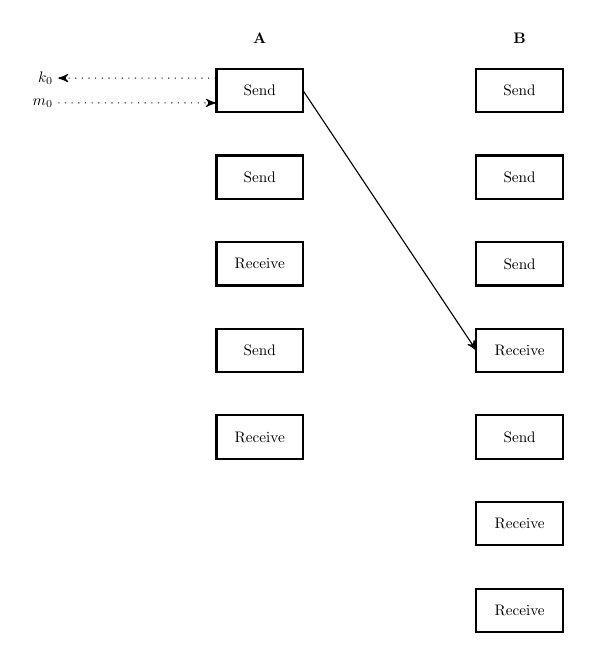
\begin{tikzpicture}[
  box/.style={rectangle,draw,inner sep=5pt,minimum height=1cm,minimum width=2cm,thick},
  node distance=2cm,
  ->,>=stealth',
  scale=0.55, every node/.style={scale=0.55}
]

  % Box t0
  \node [box] (t0) {Send};
  \node [coordinate,right of=t0,node distance=1cm] (tl0) {};
  \node [coordinate,above left=-0.125cm and 0cm of t0,node distance=1cm] (ta0) {};
  \node [left=2cm of ta0] (taa0) {$k_0$};
  \path (ta0) edge[dotted] node [] {} (taa0);
  \node [coordinate,below left=-0.125cm and 0cm of t0,node distance=1cm] (tb0) {};
  \node [left=2cm of tb0] (tbb0) {$m_0$};
  \path (tbb0) edge[dotted] node [] {} (tb0);


  \node [box,below of=t0] (t1) {Send};
  \node [box,below of=t1] (t2) {Receive};
  \node [box,below of=t2] (t3) {Send};
  \node [box,below of=t3] (t4) {Receive};

  \node [box,right of=t0,node distance=6cm] (t5) {Send};
  \node [box,below of=t5] (t6) {Send};
  \node [box,below of=t6] (t7) {Send};
  \node [box,below of=t7] (t8) {Receive};
  \node [box,below of=t8] (t9) {Send};
  \node [box,below of=t9] (t10) {Receive};
  \node [box,below of=t10] (t11) {Receive};

  \node [coordinate,left of=t8,node distance=1cm] (tl8) {};
  \path (tl0) edge[] node [] {} (tl8);

  \node [above=0.25cm of t0] (alice) {\bfseries{A}};
  \node [above=0.25cm of t5] (bob) {\bfseries{B}};
\end{tikzpicture} 
  \end{figure}
\end{frame}

\subsection{Security}
\label{sec:security}

\begin{frame}{Security I.}
  \begin{itemize}
  \item Forward security.
    \begin{itemize}
    \item Protect past states from current state leakages.
    \end{itemize}
  \item Post-compromise security (future secrecy).
    \begin{itemize}
    \item Protect future state from current state leakages.
    \end{itemize}
  \item Assert security through key- or ciphertext-indistinguishability games.
  \end{itemize}
\end{frame}

\begin{frame}{Security II.}
  \begin{figure}[ht]
      \centering
      \setlength{\fboxsep}{10pt}
      \scalebox{0.7}{%
      \fbox{%
         \algrenewcommand\textproc{}
 \algrenewcommand\algorithmicprocedure{\textbf{Game}}

 \begin{minipage}{.5\linewidth}
   \begin{algorithmic}[1]
     \Procedure{$\t{KIND}_b^\mathcal{A}$}{}
     \State $(\t{st}_\t{A},\t{st}_\t{B}) \gets$ \Call{Init}{$1^\lambda$}
     \State $b' \gets \mathcal{A}^{\t{RATCH,EXP,TEST}}$
     \State \Return $b'$
     \EndProcedure
   \end{algorithmic}
 \end{minipage}

 \vline

 \algrenewcommand\textproc{}
 \algrenewcommand\algorithmicprocedure{\textbf{Oracle}}

 \begin{minipage}{.5\linewidth}
   \begin{algorithmic}[1]
     \Procedure{TEST}{$\t{P}$}
     \If{$b = 1$}
     \State \Return $k_\t{P}$
     \EndIf
     \State \Return random $\{0,1\}^{|k_\t{P}|}$ 
     \EndProcedure

     \item[] % Blank line.

     \Procedure{EXP}{$\t{P}$}
     \State \Return $\t{st}_\t{P}$ 
     \EndProcedure
  \end{algorithmic}
\end{minipage}%

      }
    }
  \end{figure}

  \begin{figure}[ht]
      \centering
      \setlength{\fboxsep}{10pt}
      \scalebox{0.7}{%
      \fbox{%
        \algrenewcommand\textproc{}
  \algrenewcommand\algorithmicprocedure{\textbf{Game}}

  \begin{minipage}{.5\linewidth}
    \begin{algorithmic}[1]
      \Procedure{$\t{CIND}_b^\mathcal{A}$}{}
      \State $(\t{st}_\t{A},\t{st}_\t{B}) \gets$ \Call{Init}{$1^\lambda$}
      \State $b' \gets \mathcal{A}^{\t{RATCH',EXP}}$
      \State \Return $b'$
      \EndProcedure
    \end{algorithmic}
  \end{minipage}

  \vline

  \algrenewcommand\textproc{}
  \algrenewcommand\algorithmicprocedure{\textbf{Oracle}}

  \begin{minipage}{.5\linewidth}
    \begin{algorithmic}[1]
      \Procedure{RATCH'}{$\t{P},m_0,m_1$}
      \State \Return \Call{RATCH}{$\t{P},m_b$}
      \EndProcedure

      \item[] % Blank line.

      \Procedure{EXP}{$\t{P}$}
      \State \Return $\t{st}_\t{P}$ 
      \EndProcedure
   \end{algorithmic}
 \end{minipage}%

      }
    }
  \end{figure}
\end{frame}

\begin{frame}{Security III.}
  \begin{itemize}
  \item Powerful adversary.
  \item Many attacks that lead to trivial victories.
  \item Games have to be adapted to exclude these attacks.
  \item The fewer attacks a game disallows the securer the protocol.
  \item Assess advantage of any adversary.
\[
  \t{Adv}(\mathcal{A}) = \left| \Pr \left[ \t{\{C,K\}IND}_0^\mathcal{A} \rightarrow 1 \right] -
                                \Pr \left[ \t{\{C,K\}IND}_1^\mathcal{A} \rightarrow 1 \right]
                         \right|.
\]
  \end{itemize}
\end{frame}

\section{Protocols}
\label{sec:protocols}

\subsection{Timeline}
\label{sec:timeline}

\begin{frame}{Timeline I.}
  \begin{enumerate}
  \item \textbf{2012.} Off-the-record messaging protocol.
  \item \textbf{2014.} Signal protocol.
  \item \textbf{2017.} Security analysis of Signal.
  \item \textbf{2017.} Bellare {\em et al.} Formalization of ratcheting. First
    limited, unidirectional protocol.
  \end{enumerate}
\end{frame}

\begin{frame}{Timeline II.}
  \begin{enumerate}
  \item[5.] \textbf{05/2018.} Poettering and Rösler. Optimally secure bidirectional
    key-agreement protocol (BRKE).
  \item[6.] \textbf{06/2018.} Jager and Stepanovs. Optimally secure messaging protocol.
  \item[7.] \textbf{09/2018.} Durak and Vaudenay. Sub-optimally secure, efficient key-agreement
    protocol (BARK).
  \item[8.] \textbf{10/2018.} Jost, Maurer and Mularczyk. Almost-optimally secure messaging
    protocol.
  \item[9.] \textbf{10/2018.} Alwen, Coretti and Dodis. Modularization of Signal Double
    Ratchet.
  \end{enumerate}
\end{frame}

\subsection{BRKE (Poettering and Rösler)}
\label{sec:brke-poett-rosl}

\begin{frame}{BRKE (Poettering and Rösler) I.}
  \begin{itemize}
  \item Optimally secure key-agreement protocol.
    \begin{itemize}
    \item Post-impersonation authenticity.
    \item Post-impersonation confidentiality.
    \end{itemize}
  \item Leverages hierarchical identity-based encryption scheme,
    causing efficiency degradation.
  \end{itemize}
\end{frame}

\begin{frame}{BRKE (Poettering and Rösler) II.}
  The HIBE is used the mount a key-updatable key encapsulation mechanism (ku-KEM).
  \begin{align*}
    \texttt{Gen} & : \ \rightarrow \mathcal{SK} \times \mathcal{VK} \\
    \texttt{Enc} & : \mathcal{PK} \rightarrow \mathcal{K} \times \mathcal{C} \\ 
    \texttt{Dec} & : \mathcal{SK} \times \mathcal{C} \rightarrow \mathcal{K} \\
    \texttt{UpdPk} & : \mathcal{PK} \times \Delta \rightarrow \mathcal{PK} \\
    \texttt{UpdSk} & : \mathcal{SK} \times \Delta \rightarrow \mathcal{SK}
  \end{align*}
  The protocol further requires a digital signature scheme DS and a random
  oracle H.
\end{frame}

\begin{frame}{BRKE (Poettering and Rösler) III.}
  \scriptsize
   \begin{minipage}[h]{0.59\textwidth}
      \begin{figure}[h]
        \centering
        \setlength{\fboxsep}{10pt}
        \scalebox{0.7}{%
        \fbox{%
          \algrenewcommand\textproc{}
\algrenewcommand\algorithmicprocedure{\textbf{func}}

\begin{minipage}{1\linewidth}
  {\fontsize{8}{10}\selectfont

  \begin{algorithmic}[1]
    \Procedure{Init}{$K_\t{A},K_\t{B}$}
    \For{$u \in \{A,B\}$}
    \State $(sgk_\t{u},vfk_\t{u}) \gets$ \Call{\texttt{DS.Gen}}{}
    \State $(sk_\t{u},pk_\t{u}) \gets$ \Call{\texttt{ku-KEM.Gen}}{}
    \State $E^\vdash \gets 0, \ E^\dashv \gets 0$
    \State $s \gets 0, \ r \gets 0, \ t \gets \perp$
    \State $PK_\t{u}[0] \gets pk, \ SK_\t{u}[0] \gets sk$
    \State $L_\t{S}[0] \gets \perp, \ L_\t{R}[0] \gets \perp$
    \State $S_\t{u} \gets (PK_{\bar{\t{u}}},E,s,L_\t{S},
                          vfk_{\bar{\t{u}}},K_{\bar{\t{u}}},t)$
    \State $R_\t{u} \gets (SK_\t{u},E,r,L_\t{R},sgk_\t{u},K_\t{u},t)$
    \State $ST_\t{u} \gets (S_\t{u},R_\t{u})$
    \EndFor
    \State \Return $(ST_\t{A},ST_\t{B})$
    \EndProcedure
    
    % \item[]
    
    % \Procedure{Send}{$ST, ad$}
    % \State $(\sigma_\t{root},v,\gamma,T_\t{cur},t_\t{A}) \gets \t{st}_\t{A}$
    % \State $(R,S) \gets ST$
    % \State $(SK,E_\t{R},r,L_\t{R},sgk,K_\t{R},t_\t{R}) \gets R$
    % \State $(sgk^*,vfk^*) \gets$ \Call{\texttt{DS.Gen}}{}
    % \State $(sk^*,pk^*) \gets$ \Call{\texttt{DS.Gen}}{}
    % \State $E_\t{R}^\vdash \gets E_\t{R}^\vdash+1, \ SK[E_\t{R}^\vdash] \gets sk^*$
    % \State $C \gets r || pk^* || vfk^*$
    % \State $(PK,E_\t{S},s,L_\t{S},vfk,K_\t{S},t_\t{S}) \gets S$
    % \State $k^* \gets \perp, \ C \gets C || E_\t{S}^\dashv$
    % \For{$e' \gets E_\t{S}^\vdash$ to $E_\t{S}^\dashv$}
    % \State $(k,c) \gets$ \Call{\texttt{KEM.Enc}}{$PK[e']$}
    % \State $k^* \gets k^* || k, \ C \gets C || c$ 
    % \EndFor
    % \State $\sigma \gets$ \Call{\texttt{DS.Sign}}{$sgk,ad||C$}
    % \State $C \gets C || \sigma, \ L_\t{R}[E_\t{R}^\dashv] \gets ad||C$
    % \State $R \gets (SK,E_\t{R},r,L_\t{R},sgk^*,K_\t{R},t_\t{R})$
    % \State $t_\t{S} \gets ad||C$
    % \State $k.o || K_\t{S} || k.m || sk \gets$ \Call{\texttt{H}}{$K_\t{S},k^*,L_\t{S}$}
    % \State $pk \gets$ \Call{\texttt{ku-KEM.Gen}}{$sk$}
    % \State $PK[...,(E_\t{S}^\dashv -1)] \gets \perp, \ PK[E_\t{S}^\dashv] \gets pk$
    % \State $E_\t{S}^\vdash \gets E_\t{S}^\dashv, \ s \gets s+1, \ L_\t{S}[s] \gets ad||C$
    % \State $S \gets (PK,E_\t{S},s,L_\t{S},vfk,K_\t{S},t_\t{S})$
    % \State $ST \gets (R,S)$
    % \State \Return $(ST,k.o,C)$
    % \EndProcedure
  \end{algorithmic}
  }
\end{minipage}
% \begin{minipage}{0.5\linewidth}
%   {\fontsize{10}{12}\selectfont

%   \begin{algorithmic}[1]
%     \Procedure{Recceive}{$ST,ad,C$}
%     \State $(R,S) \gets ST$
%     \State $(PK,E_\t{S},s,L_\t{S},vfk,K_\t{S},t_\t{S}) \gets S$
%     \State $t^* \gets ad||C, \ t_\t{S} \gets t_\t{S} t^*, \ C || \sigma \gets C$
%     \State \textbf{assert} \Call{\texttt{DS.Verify}}{$vfk,ad||C,\sigma$}
%     \State $r||pk^*||vfk||C \gets C$
%     \State $L\t{S}[...,(r-1)] \gets \perp$
%     \For{$s' \gets r+1$  to $s$}
%     \State $pk^* \gets$ \Call{\texttt{ku-KEM.UpdPk}}{$pk^*,L\t{S}[s']$}
%     \EndFor
%     \State $E_\t{S}^\dashv \gets E_\t{S}^\dashv+1, \ PK[E_\t{S}^\dashv] \gets pk^*$
%     \State $S \gets (PK,E_\t{S},s,L_\t{S},vfk,K_\t{S},t_\t{S})$
%     \State $(SK,E_\t{R},r,L_\t{R},sgk,K_\t{R},t_\t{R}) \gets R$
%     \State $k^* \gets \perp, \ e||C \gets C$
%     \State $t_\t{R} \gets t_\t{R} || L_\t{R}[E_\t{R}^\vdash+1]||...||L_\t{R}[e]$
%     \State $L_\t{R}[...,e] \gets \perp$
%     \For{$e' \gets E_\t{R}^\vdash$ to $e$}
%     \State $c||C \gets C$
%     \State $k \gets$ \Call{\texttt{ku-KEM.Dec}}{$SK[e'],c$}
%     \State $k^* \gets k^* ||k$
%     \EndFor
%     \State $t_\t{R} \gets t_\t{R}||t^*$
%     \State $k.o || K_\t{S} || k.m || sk \gets$ \Call{\texttt{H}}{$K_\t{R},k^*,L_\t{R}$}
%     \State $SK[...,(e -1)] \gets \perp, \ SK[e] \gets sk$
%     \For{$e' \gets e+1$  to $E_\t{R}^\dashv$}
%     \State $SK[e'] \gets$ \Call{\texttt{ku-KEM.UpdSk}}{$SK[e'],t^*$}
%     \EndFor
%     \State $E_\t{R}^\vdash \gets e, \ r \gets r+1$
%     \State $R_\t{u} \gets (SK_\t{u},E,r,L_\t{R},sgk_\t{u},K_\t{u},t)$
%     \State $ST \gets (R,S)$
%     \State \Return $(ST,k.o)$ 
%     \EndProcedure
%   \end{algorithmic}
%   }
% \end{minipage}
        }
      }
    \end{figure}
    \end{minipage}
   \begin{minipage}[h]{0.40\textwidth}
      \begin{itemize}
      \item Key distribution.
      \item Parameter initialization.
      \end{itemize}
  \end{minipage}
\end{frame}

\begin{frame}{BRKE (Poettering and Rösler) IV.}
  \scriptsize
  \begin{figure}[h]
        \centering
        \setlength{\fboxsep}{10pt}
        \scalebox{0.6}{%
        \fbox{%
          \algrenewcommand\textproc{}
\algrenewcommand\algorithmicprocedure{\textbf{func}}

\begin{minipage}{1\linewidth}
  {\fontsize{8}{10}\selectfont

  \begin{algorithmic}[1]
    \Procedure{Send}{$ST, ad$}
    \State $(\sigma_\t{root},v,\gamma,T_\t{cur},t_\t{A}) \gets \t{st}_\t{A}$
    \State $(R,S) \gets ST$
    \State $(SK,E_\t{R},r,L_\t{R},sgk,K_\t{R},t_\t{R}) \gets R$
    \State $(sgk^*,vfk^*) \gets$ \Call{\texttt{DS.Gen}}{}
    \State $(sk^*,pk^*) \gets$ \Call{\texttt{DS.Gen}}{}
    \State $E_\t{R}^\vdash \gets E_\t{R}^\vdash+1, \ SK[E_\t{R}^\vdash] \gets sk^*$
    \State $C \gets r || pk^* || vfk^*$
    \State $(PK,E_\t{S},s,L_\t{S},vfk,K_\t{S},t_\t{S}) \gets S$
    \State $k^* \gets \perp, \ C \gets C || E_\t{S}^\dashv$
    \For{$e' \gets E_\t{S}^\vdash$ to $E_\t{S}^\dashv$}
    \State $(k,c) \gets$ \Call{\texttt{KEM.Enc}}{$PK[e']$}
    \State $k^* \gets k^* || k, \ C \gets C || c$ 
    \EndFor
    \State $\sigma \gets$ \Call{\texttt{DS.Sign}}{$sgk,ad||C$}
    \State $C \gets C || \sigma, \ L_\t{R}[E_\t{R}^\dashv] \gets ad||C$
    \State $R \gets (SK,E_\t{R},r,L_\t{R},sgk^*,K_\t{R},t_\t{R})$
    \State $t_\t{S} \gets ad||C$
    \State $k.o || K_\t{S} || k.m || sk \gets$ \Call{\texttt{H}}{$K_\t{S},k^*,L_\t{S}$}
    \State $pk \gets$ \Call{\texttt{ku-KEM.Gen}}{$sk$}
    \State $PK[...,(E_\t{S}^\dashv -1)] \gets \perp, \ PK[E_\t{S}^\dashv] \gets pk$
    \State $E_\t{S}^\vdash \gets E_\t{S}^\dashv, \ s \gets s+1, \ L_\t{S}[s] \gets ad||C$
    \State $S \gets (PK,E_\t{S},s,L_\t{S},vfk,K_\t{S},t_\t{S})$
    \State $ST \gets (R,S)$
    \State \Return $(ST,k.o,C)$
    \EndProcedure
  \end{algorithmic}
  }
\end{minipage}

        }
      }
    \end{figure}
       \begin{itemize}
       \item Protocol proceeds in epochs $(E^\vdash,E^\dashv)$.
       \item Continuous exchange of ku-KEM and DS keys.
       \item Unidirectional traffic accumulates ku-KEM keys.
       \end{itemize}


  %  \begin{minipage}[h]{0.59\textwidth}
  %   %\column{0\textwidth}
  %     \begin{figure}[h]
  %       \centering
  %       \setlength{\fboxsep}{10pt}
  %       \scalebox{0.6}{%
  %       \fbox{%
  %         \algrenewcommand\textproc{}
\algrenewcommand\algorithmicprocedure{\textbf{func}}

\begin{minipage}{1\linewidth}
  {\fontsize{8}{10}\selectfont

  \begin{algorithmic}[1]
    \Procedure{Send}{$ST, ad$}
    \State $(\sigma_\t{root},v,\gamma,T_\t{cur},t_\t{A}) \gets \t{st}_\t{A}$
    \State $(R,S) \gets ST$
    \State $(SK,E_\t{R},r,L_\t{R},sgk,K_\t{R},t_\t{R}) \gets R$
    \State $(sgk^*,vfk^*) \gets$ \Call{\texttt{DS.Gen}}{}
    \State $(sk^*,pk^*) \gets$ \Call{\texttt{DS.Gen}}{}
    \State $E_\t{R}^\vdash \gets E_\t{R}^\vdash+1, \ SK[E_\t{R}^\vdash] \gets sk^*$
    \State $C \gets r || pk^* || vfk^*$
    \State $(PK,E_\t{S},s,L_\t{S},vfk,K_\t{S},t_\t{S}) \gets S$
    \State $k^* \gets \perp, \ C \gets C || E_\t{S}^\dashv$
    \For{$e' \gets E_\t{S}^\vdash$ to $E_\t{S}^\dashv$}
    \State $(k,c) \gets$ \Call{\texttt{KEM.Enc}}{$PK[e']$}
    \State $k^* \gets k^* || k, \ C \gets C || c$ 
    \EndFor
    \State $\sigma \gets$ \Call{\texttt{DS.Sign}}{$sgk,ad||C$}
    \State $C \gets C || \sigma, \ L_\t{R}[E_\t{R}^\dashv] \gets ad||C$
    \State $R \gets (SK,E_\t{R},r,L_\t{R},sgk^*,K_\t{R},t_\t{R})$
    \State $t_\t{S} \gets ad||C$
    \State $k.o || K_\t{S} || k.m || sk \gets$ \Call{\texttt{H}}{$K_\t{S},k^*,L_\t{S}$}
    \State $pk \gets$ \Call{\texttt{ku-KEM.Gen}}{$sk$}
    \State $PK[...,(E_\t{S}^\dashv -1)] \gets \perp, \ PK[E_\t{S}^\dashv] \gets pk$
    \State $E_\t{S}^\vdash \gets E_\t{S}^\dashv, \ s \gets s+1, \ L_\t{S}[s] \gets ad||C$
    \State $S \gets (PK,E_\t{S},s,L_\t{S},vfk,K_\t{S},t_\t{S})$
    \State $ST \gets (R,S)$
    \State \Return $(ST,k.o,C)$
    \EndProcedure
  \end{algorithmic}
  }
\end{minipage}

  %       }
  %     }
  %   \end{figure}
  % \end{minipage}%
  %  \begin{minipage}[h]{0.40\textwidth}
  %   %\column{0.55\textwidth}
  %     \begin{itemize}
  %     \item Protocol proceeds in epochs $(E^\vdash,E^\dashv)$.
  %     \item Continuous exchange of ku-KEM and DS keys.
  %     \item Unidirectional traffic accumulates ku-KEM keys.
  %     \end{itemize}
  % \end{minipage}
  % %\end{columns}
\end{frame}

\begin{frame}{BRKE (Poettering and Rösler) V.}
  \scriptsize
    \begin{figure}[h]
        \centering
        \setlength{\fboxsep}{10pt}
        \scalebox{0.6}{%
        \fbox{%
          \algrenewcommand\textproc{}
\algrenewcommand\algorithmicprocedure{\textbf{func}}

\begin{minipage}{1.2\linewidth}
  {\fontsize{8}{10}\selectfont
    \begin{multicols}{2}
  \begin{algorithmic}[1]
    \Procedure{Receive}{$ST,ad,C$}
    \State $(R,S) \gets ST$
    \State $(PK,E_\t{S},s,L_\t{S},vfk,K_\t{S},t_\t{S}) \gets S$
    \State $t^* \gets ad||C, \ t_\t{S} \gets t_\t{S} t^*, \ C || \sigma \gets C$
    \State \textbf{assert} \Call{\texttt{DS.Verify}}{$vfk,ad||C,\sigma$}
    \State $r||pk^*||vfk||C \gets C$
    \State $L\t{S}[...,(r-1)] \gets \perp$
    \For{$s' \gets r+1$  to $s$}
    \State $pk^* \gets$ \Call{\texttt{ku-KEM.UpdPk}}{$pk^*,L\t{S}[s']$}
    \EndFor
    \State $E_\t{S}^\dashv \gets E_\t{S}^\dashv+1, \ PK[E_\t{S}^\dashv] \gets pk^*$
    \State $S \gets (PK,E_\t{S},s,L_\t{S},vfk,K_\t{S},t_\t{S})$
    \State $(SK,E_\t{R},r,L_\t{R},sgk,K_\t{R},t_\t{R}) \gets R$
    \State $k^* \gets \perp, \ e||C \gets C$
    \State $t_\t{R} \gets t_\t{R} || L_\t{R}[E_\t{R}^\vdash+1]||...||L_\t{R}[e]$
    \State $L_\t{R}[...,e] \gets \perp$
    \For{$e' \gets E_\t{R}^\vdash$ to $e$}
    \State $c||C \gets C$
    \State $k \gets$ \Call{\texttt{ku-KEM.Dec}}{$SK[e'],c$}
    \State $k^* \gets k^* ||k$
    \EndFor
    \State $t_\t{R} \gets t_\t{R}||t^*$
    \State $k.o || K_\t{S} || k.m || sk \gets$ \Call{\texttt{H}}{$K_\t{R},k^*,L_\t{R}$}
    \State $SK[...,(e -1)] \gets \perp, \ SK[e] \gets sk$
    \For{$e' \gets e+1$  to $E_\t{R}^\dashv$}
    \State $SK[e'] \gets$ \Call{\texttt{ku-KEM.UpdSk}}{$SK[e'],t^*$}
    \EndFor
    \State $E_\t{R}^\vdash \gets e, \ r \gets r+1$
    \State $R_\t{u} \gets (SK_\t{u},E,r,L_\t{R},sgk_\t{u},K_\t{u},t)$
    \State $ST \gets (R,S)$
    \State \Return $(ST,k.o)$ 
    \EndProcedure
  \end{algorithmic}
  \end{multicols}
  }
\end{minipage}
        }
      }
   \end{figure}
       \begin{itemize}
       \item Key-updates for deferred messages.
       \item Communication transcript is accumulated.
       \end{itemize}
\end{frame}

\subsection{Secure Channel (Jaeger and Stepanovs)}
\label{sec:secure-chann-jaeg}

\begin{frame}{Secure Channel (Jaeger and Stepanovs) I.}
  \begin{itemize}
  \item Optimally secure messaging protocol.
  \item Also uses HIBE scheme to provide provide key-update
    functionalities.
  \end{itemize}
\end{frame}

\begin{frame}{Secure Channel (Jaeger and Stepanovs) II.}
  The HIBE is used to build a key-updatable public-key encryption scheme (ku-PKE).
  \begin{align*}
    \texttt{Gen} & : \ \rightarrow \mathcal{DK} \times \mathcal{EK} \\
    \texttt{Enc} & : \mathcal{EK} \times \mathcal{M} \rightarrow \mathcal{C} \\
    \texttt{Dec} & : \mathcal{DK} \times \mathcal{C} \rightarrow \mathcal{M} \\
    \texttt{UpdEk} & : \mathcal{EK} \times \Delta \rightarrow \mathcal{EK} \\
    \texttt{UpdDk} & : \mathcal{DK} \times \Delta \rightarrow \mathcal{DK}
  \end{align*}
\end{frame}

\begin{frame}{Secure Channel (Jaeger and Stepanovs) III.}
  It further needs a key-updatable digital signature scheme (ku-DS).
  \begin{align*}
    \texttt{Gen} & \  \rightarrow \mathcal{SK} \times \mathcal{VK} \\
    \texttt{Sign} & : \mathcal{SK} \times \mathcal{M} \rightarrow \Sigma \\
    \texttt{Verify} & : \mathcal{VK} \times \mathcal{M} \times \Sigma \rightarrow \{0,1\} \\
    \texttt{UpdSk} & : \mathcal{SK} \times \Delta \rightarrow \mathcal{SK} \\
    \texttt{UpdVk} & : \mathcal{VK} \times \Delta \rightarrow \mathcal{VK}
  \end{align*}
  Unlike the ku-PKE the ku-DS is mounted by forward-secure signature scheme.
  We also need a collision-resistant hash function H.
\end{frame}

\begin{frame}{Secure Channel (Jaeger and Stepanovs) IV.}
  \scriptsize
  \begin{minipage}[h]{0.65\textwidth}
      \begin{figure}[h]
        \centering
        \setlength{\fboxsep}{10pt}
        \scalebox{0.7}{%
        \fbox{%
          \algrenewcommand\textproc{}
\algrenewcommand\algorithmicprocedure{\textbf{func}}

\begin{minipage}{1\linewidth}
  {\fontsize{8}{10}\selectfont

  \begin{algorithmic}[1]
    \Procedure{Init}{}
    \State $(sk_\t{I},vk_\t{R}) \gets \texttt{ku-DS.Gen}$
    \State $(ek_\t{I},dk_\t{R}[0]) \gets \texttt{ku-PKE.Gen}$
    \State $(sk_\t{R},vk_\t{I}) \gets \texttt{ku-DS.Gen}$
    \State $(ek_\t{R},dk_\t{I}[0]) \gets \texttt{ku-PKE.Gen}$
    \State $st_\t{I} \gets \t{H.Gen}, \ T_\t{R} \gets [\cdot], \ T_\t{S}[0] \gets \perp$
    \State $s \gets 0, \ r \gets 0, \ r^\t{ack} \gets 0$
    \State $st_\t{I} \gets (s,r,r^\t{ack},sk_\t{I},vk_\t{I},ek_\t{I},dk_\t{I},hk,T_\t{R},T_\t{S})$
    \State $st_\t{R} \gets (s,r,r^\t{ack},sk_\t{R},vk_\t{R},ek_\t{R},dk_\t{R},hk,T_\t{R},T_\t{S})$
    \EndProcedure
  \end{algorithmic}
  }
\end{minipage}
        }
      }
    \end{figure}
    \end{minipage}
  \begin{minipage}[h]{0.34\textwidth}
      \begin{itemize}
      \item Key distribution.
      \item Parameter initialization.
      \end{itemize}
    \end{minipage}
\end{frame}

\begin{frame}{Secure Channel (Jaeger and Stepanovs) V.}
  \scriptsize
  \begin{minipage}[ht]{0.59\textwidth}
      \begin{figure}[ht]
        \centering
        \setlength{\fboxsep}{10pt}
        \scalebox{0.7}{%
        \fbox{%
          \algrenewcommand\textproc{}
\algrenewcommand\algorithmicprocedure{\textbf{func}}

\begin{minipage}{1\linewidth}
  {\fontsize{8}{10}\selectfont
  \begin{algorithmic}[1]
    \Procedure{Send}{$st, ad,m$}
    \State $(s,r,r^\t{ack},sk,vk,ek,dk,hk,T_\t{R},T_\t{S}) \gets st$
    \State $s \gets s+1$
    \State $(sk',vk') \gets \texttt{ku-DS.Gen}$
    \State $(ek',dk[s]) \gets \texttt{ku-PKE.Gen}$
    \State $l \gets (s,r,ad,vk',ek',T_\t{R},T_\t{S}[s-1])$
    \State $ek' \gets ek$
    \For{$i \gets r^\t{ack}+1$ to $s$}
    \State $ek' \gets$ \Call{\texttt{ku-PKE.UpdEk}}{$ek', T_\t{S}[i]$}
    \EndFor
    \State $c' \gets$ \Call{\texttt{ku-PKE.Enc}}{$ek',l,m,T_\t{S}$}
    \State $v \gets (c',l), \ \sigma \gets \texttt{ku-DS.Sign}(sk,v)$
    \State $c \gets (\sigma,v), \ T_\t{S}[s] \gets \texttt{H}(hk,c)$
    \State $st \gets (s,r,r^\t{ack},sk',vk,ek,dk,hk,T_\t{R},T_\t{S})$
    \State \Return $(st,c)$
    \EndProcedure
  \end{algorithmic}
  }
\end{minipage}

        }
      }
    \end{figure}
    \end{minipage}
  \begin{minipage}[ht]{0.40\textwidth}
    %\column{0.5\textwidth}
      \begin{itemize}
      \item Continuous exchange of ku-PKE and ku-DS keys.
      \item Unidirectional traffic induces ku-PKE updates
        and accumulates decryption keys.
      \end{itemize}
    \end{minipage}
\end{frame}

\begin{frame}{Secure Channel (Jaeger and Stepanovs) VI.}
  \scriptsize
  \begin{minipage}[h]{0.65\textwidth}
  % \begin{columns}
  %  \column{0.6\textwidth}
      \begin{figure}[ht]
        \centering
        \setlength{\fboxsep}{10pt}
        \scalebox{0.7}{%
        \fbox{%
          \algrenewcommand\textproc{}
\algrenewcommand\algorithmicprocedure{\textbf{func}}

\begin{minipage}{1\linewidth}
  {\fontsize{8}{10}\selectfont
  \begin{algorithmic}[1]
    \Procedure{Receive}{$st,ad,c$}
    \State $(s,r,r^\t{ack},sk,vk,ek,dk,hk,T_\t{R},T_\t{S}) \gets st$
    \State $(\sigma,v) \gets c, \ (c',l) \gets v$
    \State $(s',r',ad',vk',ek',T_\t{R}',T_\t{S}') \gets l$
    \State $vk'' \gets vk$
    \For{$i \gets r^\t{ack}+1$ to r'}
    \State $vk'' \gets$ \Call{\texttt{ku-DS.UpdVk}}{$vk'', T_\t{S}[i]$}
    \EndFor
    \State \textbf{assert} \Call{\texttt{ku-DS.Verify}}{$vk'',\sigma,v,T_\t{S}$}
    \State $r \gets r+1, \ r^\t{ack} \gets r'$
    \State $m \gets \texttt{ku-PKE.Dec}(dk[r^\t{ack}],l,c')$
    \State $T_\t{S}[...,r^\t{ack}] \gets \perp, \ dk_\t{S}[...,r^\t{ack}] \gets \perp$
    \State $T_\t{R} \gets \texttt{H}(hk,c), \ sk \gets \texttt{ku-DS.UpdSk}(sk,T_\t{R})$
    \For{$i = r^\t{ack}$ to $s$}
    \State $dk[i] \gets$ \Call{\texttt{ku-PKE.UpdDk}}{$dk[i],T_\t{R}$}
    \EndFor
    \State $st \gets (s,r,r^\t{ack},sk,vk',ek',dk,hk,T_\t{R},T_\t{S})$
    \State \Return $(st,m)$
    \EndProcedure
  \end{algorithmic}
  }
\end{minipage}
        }
      }
    \end{figure}
    \end{minipage}
  \begin{minipage}[h]{0.34\textwidth}
   % \column{0.5\textwidth}
      \begin{itemize}
      \item ku-DS signing key is always updated.
      \item $r^\t{ack}$ designates number of acknowledged messages.
      \end{itemize}
    \end{minipage}
\end{frame}

\subsection{BARK (Durak and Vaudenay)}
\label{sec:bark-durak-vaudenay}

\begin{frame}{BARK (Durak and Vaudenay) I.}
  \begin{itemize}
  \item Sub-optimally secure but very efficient key-agreement protocol.
  \item Relies only on regular public-key cryptosystems.
  \item Recover security.
  \item Composed of a simpler unidirectional messaging protocol (uniARCAD),
    one instance per user.
  \end{itemize}
\end{frame}

\begin{frame}{BARK (Durak and Vaudenay) II.}
  BARK relies on a simple signcryption construction, combining a public-key
  encryption scheme and digital signature scheme.
  \begin{align*}
    \texttt{PKE.Gen} & : \ \rightarrow \mathcal{SK}_\t{R} \times \mathcal{PK}_\t{R} \\
    \texttt{DS.Gen} & : \ \rightarrow \mathcal{SK}_\t{S} \times \mathcal{PK}_\t{S} \\
    \texttt{Enc} & : \mathcal{SK}_\t{S} \times \mathcal{PK}_\t{R} \times \mathcal{M} \times
                   \mathcal{AD} \rightarrow \mathcal{C} \\
    \texttt{Dec} & : \mathcal{SK}_\t{R} \times \mathcal{PK}_\t{S} \times
  \mathcal{C} \times \mathcal{AD} \rightarrow \mathcal{M}
  \end{align*}
  It further needs some collision-resistant hash function H.
\end{frame}

\begin{frame}{BARK (Durak and Vaudenay) III.}
   \begin{figure}[h]
     \centering
     \setlength{\fboxsep}{10pt}
     \scalebox{0.7}{%
       \fbox{%
          \algrenewcommand\textproc{}
\algrenewcommand\algorithmicprocedure{\textbf{func}}

\begin{minipage}{.5\linewidth}
  {\fontsize{8}{10}\selectfont

    \begin{algorithmic}[1]
    \Procedure{Init}{}
    \State $(sk_\t{S},pk_\t{S}) \gets$ \Call{\texttt{PKE.Gen}}{}
    \State $(sk_\t{R},pk_\t{R}) \gets$ \Call{\texttt{DS.Gen}}{}

    \State $st_\t{S} \gets (sk_S,pk_\t{R})$ 
    \State $st_\t{R} \gets (sk_R,pk_\t{S})$ 

    \State \Return $(st_\t{S},st_\t{R})$
    \EndProcedure
    \end{algorithmic}

    \vspace{10pt}

    \begin{algorithmic}[1]
    \Procedure{Receive}{$st_\t{R}, ad, ct$}
    \State $(sk_\t{R},pk_\t{S}) \gets st_\t{R}$ 
    \State $pt' \gets$ \Call{\texttt{Dec}}{$sk_\t{R},pk_\t{S},ad,ct$}
    \If{$pt' = \perp$}
    \State \Return $(\t{false}, st_\t{R}, \perp)$
    \EndIf
    \State $(pt,st_\t{R}') \gets pt'$
    \State \Return $(\t{true},st_\t{R}, pt)$
    \EndProcedure
   
  \end{algorithmic}
  }
\end{minipage}

\begin{minipage}{.5\linewidth}
  {\fontsize{8}{10}\selectfont

  \begin{algorithmic}[1]
    \Procedure{Send}{$st_\t{S}, ad, pt, \t{flag}$}
    \State $(sk_\t{S},pk_\t{R}) \gets st_\t{S}$ 
    \If{$\t{flag} = \t{true}$}
    \State $(sk_\t{S}',pk_\t{S}') \gets$ \Call{\texttt{PKE.Gen}}{}
    \State $(\t{sk}_\t{R}',\t{pk}_\t{R}') \gets$ \Call{\texttt{DS.Gen}}{}
    \State $st_\t{S}' \gets (sk_\t{S}',pk_\t{R}')$
    \State $st_\t{R}' \gets (sk_\t{R}',pk_\t{S}')$
    \Else
    \State $(sk_\t{S}',pk_\t{R}') \gets (\perp,\perp)$
    \EndIf
    \State $pt' \gets st_\t{R}' || pt$
    \State $ct \gets$ \Call{\texttt{Enc}}{$sk_\t{S},pk_\t{R}, ad, pt'$}
    \State \Return $(st_\t{S}', ct)$
    \EndProcedure
    
  \end{algorithmic}
  }
\end{minipage}

       }
     }
  \end{figure}
\end{frame}

\begin{frame}{BARK (Durak and Vaudenay) IV.}
   \scriptsize
  \begin{minipage}[h]{0.49\textwidth}
  % \begin{columns}
  %  \column{0.6\textwidth}
      \begin{figure}[ht]
        \centering
        \setlength{\fboxsep}{10pt}
        \scalebox{0.7}{%
        \fbox{%
          \algrenewcommand\textproc{}
\algrenewcommand\algorithmicprocedure{\textbf{func}}

\begin{minipage}{\linewidth}
  {\fontsize{8}{10}\selectfont
  \begin{algorithmic}[1]
    \Procedure{Init}{}
    \State $(st_\t{A}^\t{send},st_\t{B}^\t{rec}) \gets$ \Call{\texttt{uniBARK.Init}}{}
    \State $(st_\t{B}^\t{send},st_\t{A}^\t{rec}) \gets$ \Call{\texttt{uniBARK.Init}}{}
    \State pick $hk$ at random
    \State $st_\t{A} \gets (hk, [st_\t{A}^\t{send}], [st_\t{A}^\t{rec}],\perp,\perp)$ 
    \State $st_\t{B} \gets (hk, [st_\t{B}^\t{send}], [st_\t{B}^\t{rec}],\perp,\perp)$ 
    \State \Return $(st_\t{A},st_\t{B})$
    \EndProcedure
  \end{algorithmic}
  }
\end{minipage}

        }
      }
    \end{figure}
    \end{minipage}
  \begin{minipage}[h]{0.49\textwidth}
   % \column{0.5\textwidth}
      \begin{itemize}
      \item Initialize two uniARCAD instances and distribute the
        resulting states.
      \item Further initialize two variables (Hsent, Hreceived) to $\perp$ which will
        hold the chain-hash of all sent and received messages.
      \end{itemize}
    \end{minipage}
  \end{frame}

\begin{frame}{BARK (Durak and Vaudenay) V.}
  \scriptsize
  \begin{figure}[ht]
     \centering
     \setlength{\fboxsep}{10pt}
     \scalebox{0.5}{%
       \fbox{%
         \algrenewcommand\textproc{}
\algrenewcommand\algorithmicprocedure{\textbf{func}}

\begin{minipage}{\linewidth}
  {\fontsize{8}{10}\selectfont
  \begin{algorithmic}[1]
    \Procedure{Send}{$st_\t{P}$}
    \State pick $k$ at random
    \State $(hk, [st_\t{P}^\t{send,1},...,st_\t{P}^\t{send,u}],
                 [st_\t{P}^\t{rec,1},...,st_\t{P}^\t{rec,v}],
    \t{Hsent}, \t{Hreceived}) \gets st_\t{P}$
    \State $(st_\t{S,new},st_\t{P}^\t{rec,v+1}) \gets$ \Call{\texttt{uniARCAD.Init}}{}
    \State $\t{onion} \gets st_\t{S,new} || k$
    \State find smallest i such that $st_\t{P}^\t{send,i} \neq \perp$
    \For{$j \gets u$ to $i$}
    \State $(st_\t{P}^\t{send,j},\t{onion}) \gets$ \Call{\texttt{uniARCAD.Send}}
               {$st_\t{P}^\t{send,j},(u-j)||\t{onion},j=u$}
    \If{$j < u$}
    \State $st_\t{P}^\t{send,j} \gets \perp$
    \EndIf
    \EndFor

    \State $\t{upd} \gets (u-i)||\t{Hsent}||\t{onion}$
    \State $\t{Hsent}' \gets$ \Call{\texttt{H}}{hk,\t{upd}}
    \State $st_\t{P}' \gets (hk,[st_\t{P}^\t{send,1},...,st_\t{P}^\t{send,u}],
                 [st_\t{P}^\t{rec,1},...,st_\t{P}^\t{rec,v+1}], \t{Hsent}', \t{Hreceived})$

    \State \Return $(st_\t{P}', \t{upd})$
    \EndProcedure
  \end{algorithmic}
  }
\end{minipage}

       }
     }
  \end{figure}
  \begin{itemize}
  \item Continuously exchange signcryption keys.
  \item First message in the other direction after unidirectional traffic
    will use all accumulated keys in the onion encryption.
  \item Chain-hash ensures recover security.
  \end{itemize}
\end{frame}

\begin{frame}{BARK (Durak and Vaudenay) VI.}
  \scriptsize
  \begin{figure}[ht]
     \centering
     \setlength{\fboxsep}{10pt}
     \scalebox{0.5}{%
       \fbox{%
         \algrenewcommand\textproc{}
\algrenewcommand\algorithmicprocedure{\textbf{func}}

\begin{minipage}{\linewidth}
  {\fontsize{8}{10}\selectfont
  \begin{algorithmic}[1]
    \Procedure{Receive}{$st_\t{P}, \t{upd}$}
    \State $(hk, [st_\t{P}^\t{send,1},...,st_\t{P}^\t{send,u}],
                 [st_\t{P}^\t{rec,1},...,st_\t{P}^\t{rec,v}],
    \t{Hsent}, \t{Hreceived}) \gets st_\t{P}$
    \State $(n,h,\t{onion}) \gets \t{upd}$
    \If{$h \neq \t{Hreceived}$}
    \State \Return $(\t{false},st_\t{P},\perp)$
    \EndIf
    \State find smallest i such that $st_\t{P}^\t{rec,i} \neq \perp$
    \For{$j \gets i$ to $i+n$}
    \State $(\t{acc},st_\t{P}^\t{rec,j'},\t{onion}) \gets$ \Call{\texttt{uniARCAD.Receive}}
    {$st_\t{P}^\t{rec,j}$}
    \If{$\t{acc} = \t{false}$}
    \State \Return $(\t{false},st_\t{P},\perp)$
    \EndIf
    \EndFor

    \State $(st_\t{P}^\t{send,u+1},k) \gets \t{onion}$
    \For{$j \gets i$ to $i+n-1$}
    \State $st_\t{P}^\t{rec,j} \gets \perp$
    \EndFor
    \State $st_\t{P}^\t{rec,i+n} \gets st_\t{P}^\t{rec,i+n'}$
    \State $\t{Hreceived}' \gets$ \Call{\texttt{H}}{$hk,\t{upd}$}
    \State $st_\t{P}' \gets (hk,[st_\t{P}^\t{send,1},...,st_\t{P}^\t{send,u+1}],
                 [st_\t{P}^\t{rec,1},...,st_\t{P}^\t{rec,v}], \t{Hsent}, \t{Hreceived}')$

    \State \Return $(\t{true}, st_\t{P}',k)$
    \EndProcedure
  \end{algorithmic}
  }
\end{minipage}

       }
     }
  \end{figure}
  \begin{itemize}
  \item Accumulate received signcryption keys for responding.
  \item Use all accumulated keys when receiving message
  \item All the accumulated keys will be used in when responding.
  \end{itemize}
\end{frame}

\subsection{Secure Channel (Jost, Maurer \& Mularczyk)}
\label{sec:secure-channel-jost}

\begin{frame}{Secure Channel (Jost, Maurer \& Mularczyk) I.}
  \begin{itemize}
  \item Aims to fill the gap between BARK and the first two protocols.
  \item Almost completely post-impersonation secure but less efficient than BARK.
  \item As BARK only relies on regular public-key cryptosystems however
    it proposes several rather complicated key-update primitives.
  \end{itemize}
\end{frame}

\begin{frame}{Secure Channel (Jost, Maurer \& Mularczyk) II.}
  The first primitive is a key-updatable signature scheme (ku-Sig).
  \begin{align*}
    \texttt{Gen} & : \ \rightarrow \mathcal{VK} \times \mathcal{SK} \\
    \texttt{Sign} & : \mathcal{SK} \times \mathcal{M} \rightarrow \mathcal{SK} \times \Sigma \\
    \texttt{Verify} & : \mathcal{VK} \times \mathcal{M} \times \Sigma
             \rightarrow \mathcal{VK} \times \{0,1\}
  \end{align*}
A ku-Sig can be constructed out of a regular digital signature scheme.
\end{frame}

\begin{frame}{Secure Channel (Jost, Maurer \& Mularczyk) III.}
  The protocol further needs a secretly key-updatable public-key encryption scheme (sku-PKE).
   \begin{align*}
     \texttt{Gen} & : \ \rightarrow \mathcal{EK} \times \mathcal{DK}, \
     && \texttt{UpdGen} : \ \rightarrow \mathcal{UE} \times \mathcal{UD} \\
     \texttt{Enc} & : \mathcal{EK} \times \mathcal{M} \rightarrow \mathcal{C}, \
     && \texttt{UpdEk} : \mathcal{UE} \times \mathcal{EK} \rightarrow \mathcal{EK} \\
     \texttt{Dec} & : \mathcal{DK} \times \mathcal{C} \rightarrow \mathcal{M}, \
     && \texttt{UpdDk} :  \mathcal{UD} \times \mathcal{DK} \rightarrow \mathcal{DK}
  \end{align*}
The update information is independently generated and the keys
can be separately updated. A sku-PKE can be mounted with the
components of the ElGamal cryptosystem.
\end{frame}

\begin{frame}{Secure Channel (Jost, Maurer \& Mularczyk) IV.}
  The sku-PKE serves as a building block a healable and key-updating
  public-key encryption scheme (hku-PKE). We further need a regular
  PKE that can treat associated data (PKE-AD).
  \begin{align*}
    \texttt{Gen} & : \ \rightarrow \mathcal{EK} \times \mathcal{DK}, \ &&
    \texttt{BcUpEk} : \mathcal{EK} \times \Delta \rightarrow \mathcal{EK} \\
    \texttt{Enc} & : \mathcal{EK} \times \mathcal{M} \times \mathcal{AD}
                   \rightarrow \mathcal{C}, \ &&
    \texttt{BcUpDk} : \mathcal{DK} \times \Delta \rightarrow \mathcal{DK} \\
    \texttt{Dec} & : \mathcal{DK} \times \mathcal{C} \times \mathcal{AD}
                   \rightarrow \mathcal{M}
  \end{align*}
  Update calls do not to be synchronized anymore, meaning that decryption still
  succeeds for any sequence of \texttt{BcUpDk} call even if only a prefix
  of the used update information has been used in \texttt{BcUpEk} calls.
\end{frame}

\begin{frame}{Secure Channel (Jost, Maurer \& Mularczyk) V.}
  \scriptsize
  \begin{figure}[ht]
     \centering
     \setlength{\fboxsep}{10pt}
     \scalebox{0.6}{%
       \fbox{%
         \algrenewcommand\textproc{}
\algrenewcommand\algorithmicprocedure{\textbf{func}}
\begin{minipage}{\linewidth}
  {\fontsize{10}{12}\selectfont
  \begin{algorithmic}[1]
    \Procedure{Init}{}
    \For{$u \in \{A,B\}$}
      \State $(ek_u,dk_u) \gets$ \Call{\texttt{hku-PKE.Gen}}{}
      \State $(sk_u^\t{upd},vk_u^\t{upd}) \gets$ \Call{\texttt{ku-Sig.Gen}}{}
      \State $(sk_u^\t{eph},vk_u^\t{eph}) \gets$ \Call{\texttt{Sig.Gen}}{}
    \EndFor
    \For{$u \in \{A,B\}$}
    \State $st_u \gets (0,0,0,dk_u,ek_{\bar{u}},sk_u^\t{upd},vk_{\bar{u}}^\t{upd},
                        sk_u^\t{eph},vk_{\bar{u}}^\t{ep},[\cdot],\perp,[\cdot])$
    \EndFor
    \State \Return $(st_\t{A},st_\t{B})$
    \EndProcedure
   \end{algorithmic}
  }
\end{minipage}

       }
     }
  \end{figure}
  \begin{itemize}
  \item Protocol also needs a regular digital signature scheme (Sig).
  \item Generate two key pairs for each primitive and distribute them to the users.
  \item Further initialize a Sig verification key array $VK^\t{eph}$, a transcript
    variable holding the chain-hash of the messages $tr$ and a transcript array $TR$.
  \end{itemize}
\end{frame}

\begin{frame}{Secure Channel (Jost, Maurer \& Mularczyk) VI.}
  \scriptsize
  \begin{figure}[ht]
     \centering
     \setlength{\fboxsep}{10pt}
     \scalebox{0.6}{%
       \fbox{%
         \algrenewcommand\textproc{}
\algrenewcommand\algorithmicprocedure{\textbf{func}}
\begin{minipage}{\linewidth}
  {\fontsize{10}{12}\selectfont
  \begin{algorithmic}[1]
    \Procedure{Send}{$st,m$}
    \State $(r,s,s_\t{ack},dk,ek,sk^\t{upd},vk^\t{upd},
                        sk^\t{eph},vk^\t{eph},VK^\t{eph},tr,TR) \gets st$
    \State $(sk_1^\t{eph},vk_1^\t{eph}) \gets$ \Call{\texttt{Sig.Gen}}{}
    \State $(sk_2^\t{eph},vk_2^\t{eph}) \gets$ \Call{\texttt{Sig.Gen}}{}

    \State $(dk,upd) \gets$ \Call{\texttt{hku-PKE.BcUpDk}}{$dk$}
    \State $c \gets$ \Call{\texttt{hku-PKE.Enc}}{$ek,m||sk_1^\t{eph},upd||vk_2^\t{eph}||r$}
    \State $c' \gets c||upd||vk_2^\t{eph}||r$
    \State $(sk^\t{upd},\sigma_\t{upd}) \gets$ \Call{\texttt{ku-Sig.Sign}}{$sk^\t{upd},c'||tr$}
    \State $\sigma_\t{eph} \gets$ \Call{\texttt{Sig.Sign}}{$sk^\t{eph},c'||tr$}

    \State $s \gets s+1$
    \State $VK[s] \gets vk_1^\t{eph}$
    \State $TR[s] \gets$ \Call{\texttt{H}}{$Tr[s-1]||c'$}
    
    
    \State $st \gets (r,s,s_\t{ack},dk,ek,sk^\t{upd},vk^\t{upd},
                        sk_2^\t{eph},vk^\t{ep},VK^\t{eph},tr,TR)$
    
    \State \Return $(st, (c',\sigma_\t{upd},\sigma_\t{eph}))$
    \EndProcedure
   \end{algorithmic}
  }
\end{minipage}

       }
     }
  \end{figure}
  \begin{itemize}
  \item Generate two sets of Sig key pairs for sending and receiving and
    accumulate the verification key.
  \item Update hku-PKE decryption key for each message.
  \item Combination of ku-Sig and Sig signature yields post-impersonation
    authenticity.
  \end{itemize}
\end{frame}

\begin{frame}{Secure Channel (Jost, Maurer \& Mularczyk) VII.}
  \scriptsize
  \begin{figure}[ht]
     \centering
     \setlength{\fboxsep}{10pt}
     \scalebox{0.55}{%
       \fbox{%
         \algrenewcommand\textproc{}
\algrenewcommand\algorithmicprocedure{\textbf{func}}
\begin{minipage}{\linewidth}
  {\fontsize{10}{12}\selectfont
  \begin{algorithmic}[1]
    \Procedure{Receive}{$st,ct$}
    \State $(r,s,s_\t{ack},dk,ek,sk^\t{upd},vk^\t{upd},
                        sk^\t{eph},vk^\t{eph},VK^\t{eph},tr,TR) \gets st$
    \State $(c',\sigma_\t{upd},\sigma_\t{eph}) \gets ct$
    \State $(c,upd,vk_\t{msg}^\t{eph},s_\t{msg}) \gets c'$
    \If{$s_\t{msg} > s_\t{ack}$}
    \State $vk \gets VK^\t{eph}[s_\t{msg}]$
    \Else
    \State $vk \gets vk^\t{eph}$
    \EndIf

    \State $v_\t{eph} \gets$
    \Call{\texttt{Sig.Verify}}{$vk,c'||TR[s_\t{msg}],\sigma_\t{eph}$}
    \State $(vk^\t{upd},v_\t{upd}) \gets$
    \Call{\texttt{ku-Sig.Verify}}{$vk^\t{upd},c', \sigma_\t{upd}$}
    \State \textbf{assert} $v_\t{eph} \wedge v_\t{upd}$

    \State $ek \gets$ \Call{\texttt{hku-PKE.BcUpEk}}{$ek,upd$} 
    \State $(dk, (m,sk_\t{msg}^\t{eph})) \gets$
    \Call{\texttt{hku-PKE.Dec}}{$dk,c,upd||vk_\t{msg}^\t{eph}||s_\t{msg}$}
    \State $r \gets r +1$
    \State $tr \gets$ \Call{\texttt{H}}{$tr||c'$}
    
    \State $st \gets (r,s,s_\t{msg},dk,ek,sk^\t{upd},vk^\t{upd},
                        sk_\t{msg}^\t{eph},vk_\t{msg}^\t{ep},VK^\t{eph},tr,TR)$

    \State \Return $(st,m)$
    \EndProcedure
  \end{algorithmic}
  }
\end{minipage}

       }
     }
  \end{figure}
  \begin{itemize}
  \item Update hku-PKE encryption key for each message.
  \end{itemize}
\end{frame}

\subsection{Double Ratchet (Alwen, Coretti \& Dodis)}
\label{sec:double-ratchet-alwen}

\begin{frame}{Double Ratchet (Alwen, Coretti \& Dodis)}
  
\end{frame}




\end{document}
